\documentclass{article}
\usepackage[T1]{fontenc}
\usepackage{lmodern}
\usepackage{graphicx}
\usepackage{amsmath,amssymb}
\usepackage[a4paper,margin=2cm]{geometry}
\usepackage[absolute,overlay]{textpos}
\setlength{\TPHorizModule}{1mm}
\setlength{\TPVertModule}{1mm}
\usepackage[indonesian]{babel}
\usepackage{hyperref}
\setlength{\emergencystretch}{2em}
% unit: Halaman 9

\begin{document}

% === Halaman 9 (python/native) ===

ENKRIPSI:

Plainteks: temui saya di jembatan merah nanti malam

• p1 = ‘t’ = 19 → c1 = E(19) = (19 + 3) mod 26 = 22 = ‘W’

• p2 = ‘e’ = 4  → c2 = E(4) = (4 + 3) mod 26 = 7 = ‘H’

• p3 = ‘m’ = 12 → c3 = E(12) = (12 + 3) mod 26 = 15 = ‘P’

• p4 = ‘u’ = 20 → c4 = E(20) = (20 + 3) mod 26 = 23 = ‘X’

• p5 = ‘i’ = 8 

→ c4 = E(8) = (8 + 3) mod 26 = 11 = ‘L’

• dst…

Cipherteks: 

WHPXL VDBD GL MHPEDWDQ PHUDK QDQWL PDODP

9

% deskripsi: gambar native xref 66
\noindent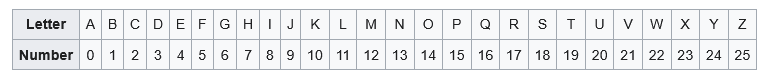
\includegraphics[width=0.85\textwidth]{../../images/python/page_009_img_01.png}

\end{document}
